\chapter{Architektur}

\section{Übersicht}

Um eine Drohne über einen Server in der Cloud steuern zu können, muss diese mit dem Internet verbunden werden. Dies ist nur über einen Proxy möglich, in diesem Fall ein Mobiltelefon. Das Mobiltelefon bietet andereseits auch eine Benutzeroberfläche um das Beladen und das Abfragen des Zustands der Drohne zu erleichtern. \\

\begin{figure}[h]
	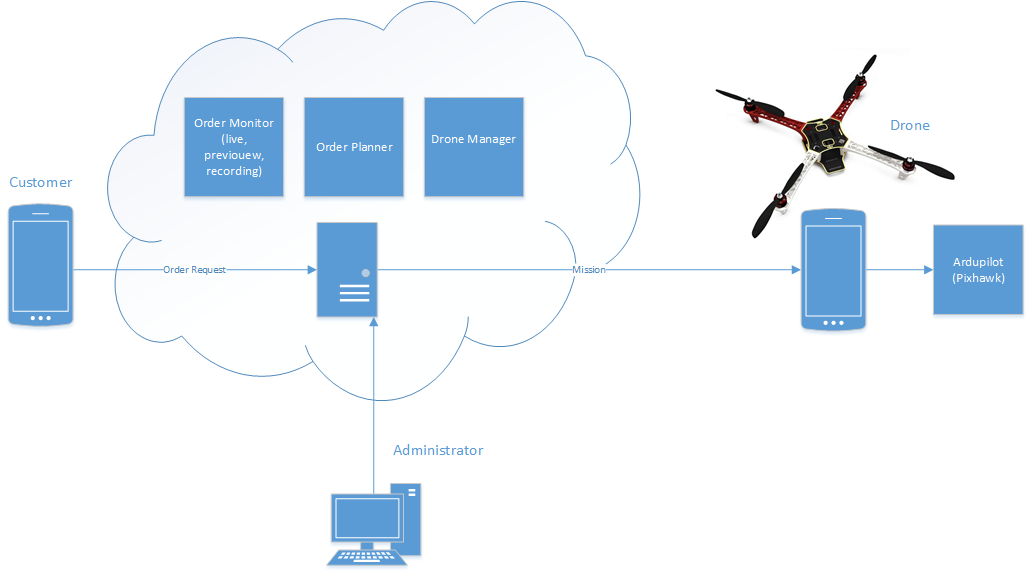
\includegraphics[width=1.0\textwidth]{images/Overview-Diagram.png}
	\caption{Übersicht der Project Helin Architektur }
	\label{fig:architecture-overview}
\end{figure}

\section{Kommunikations-Architektur}

Die Abbildung \ref{fig:communication-architecture-overview}) zeigt die Kommunikations-Architektur in der Übersicht. Wichtig sind vor allem die verschiedenen verwendeten Protokolle, die benötigt werden um die Funktionalen- und Nicht-Funktionalen-Anforderungen zu erfüllen. Bei den mobilen Geräten wird Messaging (AMQP) verwendet um bidirektionale Kommunikation zu ermöglichen. Dies ist nötig, damit Kunden und Administratoren die Bewegungen der Drohne live verfolgen können. Ausserdem bietet Messaging mit "Exactly Once" ein wichtiges Feature um die nötige Zuverlässigkeit zu gewährleisten. 


\begin{figure}[h]
	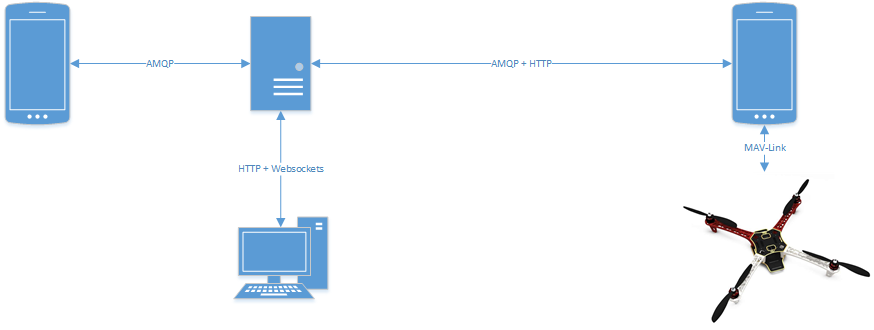
\includegraphics[width=1.0\textwidth]{images/Communication-Overview-Diagram.png}
	\caption{Übersicht der Kommunikations-Architektur mit den jeweiligen Protokollen. }
	\label{fig:communication-architecture-overview}
\end{figure}